\documentclass[12pt,a4paper]{report}

%%------------------------------- preamble ------------------------------------

%% comment next for EN
% \usepackage[portuges]{babel}      % language PT 
\usepackage[utf8]{inputenc}       % accents
\usepackage[T1]{fontenc}          % PS fonts
\usepackage{newtxtext,newtxmath}  % do not use CM fonts
\usepackage{amsmath}              % multi-line and other mathematical statements
\usepackage{setspace}             % setting the spacing between lines
\usepackage{graphicx}             % go far beyond what the graphics package
\usepackage[normalem]{ulem}       % various types of underlining
\usepackage{caption}              % rotating captions, sideways captions, etc.
\usepackage{float}                % tables and figures in the multi-column environment 
\usepackage{subcaption}           % for subfigures and the like
\usepackage{longtable}            % tables that continue to the next page
\usepackage{multirow}             % tabular cells spanning multiple rows
\usepackage{booktabs}             % to create professional-quality tables
\usepackage[table]{xcolor}        % driver-independent color extensions
\RequirePackage{xurl}             % URL-sensitive line breaks
\usepackage{lipsum}               % loren dummy text
\setlength{\marginparwidth}{2cm}  % todonotes' requirements
\usepackage{todonotes}            % todo's
\usepackage{csquotes}             % context sensitive quotation facilities
% \usepackage[backend=biber,authordate]{biblatex-chicago}  % Chicago Manual of Style
\usepackage{pgfgantt}             % Gantt charts
\usepackage[printonlyused]{acronym} % for acronyms
\usepackage{eurosym}              % for the Euro currency symbol
\usepackage{siunitx}              % for SI Unit rules and style conventions
% \sisetup{
%   group-separator = {\,},         % a thin space
%   group-minimum-digits = 4        % enable grouping for numbers ≥ 1000
% }
\DeclareSIUnit{\eurocurrency}{\text{\euro}}  % for the Euro symbol in siunitex

%% document dimensions
\usepackage[a4paper,left=25mm,right=25mm,top=25mm,bottom=25mm,headheight=6mm,
footskip=12mm]{geometry}
\setlength{\parindent}{0em}
\setlength{\parskip}{1ex}

%% headers & footers
\usepackage{lastpage}
\usepackage{fancyhdr}
\fancyhf{}                            % clear off all default fancyhdr headers and footers
\rhead{\small{\emph{\projtitle, \projauthor}}}
\rfoot{\small{\thepage\ / \pageref{LastPage}}}
\pagestyle{fancy}                     % apply the fancy header style
\renewcommand{\headrulewidth}{0.4pt}
\renewcommand{\footrulewidth}{0.4pt}

%% colors
\usepackage{color}
\definecolor{engineering}{rgb}{0.549,0.176,0.098}
\definecolor{cloudwhite}{cmyk}{0,0,0,0.025}

%% source-code listings
\usepackage{listings}
\lstset{ %
 language=C,                        % choose the language of the code
 basicstyle=\footnotesize\ttfamily,
 keywordstyle=\bfseries,
 numbers=left,                      % where to put the line-numbers
 numberstyle=\scriptsize\texttt,    % the size of the fonts that are used for the line-numbers
 stepnumber=1,                      % the step between two line-numbers. If it's 1 each line will be numbered
 numbersep=8pt,                     % how far the line-numbers are from the code
 frame=tb,
 float=htb,
 aboveskip=8mm,
 belowskip=4mm,
 backgroundcolor=\color{cloudwhite},
 showspaces=false,                  % show spaces adding particular underscores
 showstringspaces=false,            % underline spaces within strings
 showtabs=false,                    % show tabs within strings adding particular underscores
 tabsize=2,                         % sets default tabsize to 2 spaces
 captionpos=t,                      % sets the caption-position to top
 belowcaptionskip=12pt,             % space between caption and listing
 breaklines=true,                   % sets automatic line breaking
 breakatwhitespace=false,           % sets if automatic breaks should only happen at whitespace
 escapeinside={\%*}{*)},            % if you want to add a comment within your code
 morekeywords={*,var,template,new}  % if you want to add more keywords to the set
}
\lstdefinestyle{bash}{
    language=bash,
    basicstyle=\ttfamily\small,
    keywordstyle=\color{blue},
    commentstyle=\color{gray},
    stringstyle=\color{green!50!black},
    breaklines=true,
    frame=single,
    showstringspaces=false
}

%% hyperreferences (HREF, URL)
\usepackage{hyperref}
\hypersetup{
    plainpages=false, 
    pdfpagelayout=SinglePage,
    bookmarksopen=false,
    bookmarksnumbered=true,
    breaklinks=true,
    linktocpage,
    colorlinks=true,
    linkcolor=engineering,
    urlcolor=engineering,
    filecolor=engineering,
    citecolor=engineering,
    allcolors=engineering
}

%% path to the figures directory
\graphicspath{{figures/}}

%% bibliography file, must be in preamble
% \addbibresource{bibliography.bib}

%% macros to be updated as needed
\newcommand{\school}{Faculdade de Ciências da Universidade do Porto}
\newcommand{\degree}{Master in Information Security}
\newcommand{\projtitle}{Bug Bounty Project}
\newcommand{\subtitle}{Final Project Report}
%\newcommand{\subtitle}{Capstone Project Final Report}
\newcommand{\projauthor}{Tiago Almeida and Gabriel Ferreira}
% \newcommand{\supervisor}{Nome do Supervisor}
\newcommand{\tutor}{Prof.\ André Baptista e Miguel Regala}
\newcommand{\class}{Theory and Practice of Security Attacks}

%% other macros, if needed
\newcommand{\windspt}{\textsf{WindsPT\/}}
\newcommand{\windscannerpt}{\emph{Windscanner.PT\/}}
% \newcommand{\class}[1]{{\normalfont\sffamily #1\/}}
% \newcommand{\svg}{\class{SVG}}

%% environments for infos
\newenvironment{info}[1]{\vspace*{6mm}\color{blue}[ \textbf{INFO:} \begin{em} #1}{\vspace*{3mm}\end{em} ]}
\newenvironment{infoopt}[1]{\vspace*{6mm}\color{blue}[ \textbf{INFO (elemento opcional):} \begin{em} #1}{\vspace*{3mm}\end{em} ]}

%%------------------------------- document-------------------------------------

\begin{document}

%% preamble page numbers with roman numerals
\pagenumbering{roman}\setcounter{page}{1}
\pagestyle{plain}

%%------------------------------- cover page ----------------------------------

\begin{titlepage}
	\center

	\vspace{-15mm}
	{\fontsize{18}{22}\selectfont \textbf{\textsc{\school}}}\\

	\vspace{30mm}

	{\fontsize{28}{34}\selectfont \textbf{\projtitle}}\\[6mm]
	{\fontsize{18}{22}\selectfont \textbf{\subtitle}}\\[28mm]

	\vspace{10mm}

	
\includegraphics[width=150mm]{images/fcup.png}

	\vfill

	{\large \textbf{\degree}}\\[4mm]
	{\large \textbf{\class}}\\[4mm]
	{\large \textbf{Authors}: \projauthor}\\[4mm]
	{\large \textbf{Teachers}: \tutor}\\[4mm]

	%% fix date if needed
	%\renewcommand{\today}{15 de dezembro de 2023}
	\today

\end{titlepage}

%%------------------------------- Abstract ------------------------------------

\chapter*{Summary}

This report documents the work carried out by our group within the scope of the final project for the course Theory and Practice of Security Attacks, focusing on Bug Bounty Programs as a practical approach to vulnerability research. The main objective of the project was to gain hands-on experience in security testing methodologies while attempting to identify a reportable vulnerability within real-world systems.

Throughout the project, we explored multiple Bug Bounty and Vulnerability Disclosure Programs, adapting our approach as our understanding of effective reconnaissance and research techniques evolved. We began with narrowly scoped programs and progressively transitioned to broader scopes, which significantly increased the available attack surface. This shift highlighted the importance of flexibility and iterative learning in vulnerability research.

A large part of the project was dedicated to reconnaissance, including asset discovery, subdomain enumeration, technology identification, filtering, and prioritization. We relied on a combination of manual analysis and automated tools, learning from initial mistakes such as overfiltering and incorrect assumptions about target similarity. These lessons proved essential in refining our methodology and improving efficiency.

By the end of the project, we successfully identified a vulnerability within scope and reflected on the techniques, tools, and decisions that led to its discovery. Overall, this work provided valuable insight into real-world Bug Bounty workflows and strengthened our practical skills in cybersecurity research.

%\vspace{\fill}
%{\Large \textbf{Palavras-chave}:} palavra1, palavra2, palavra3, palavra4
%\vspace*{24mm}

\acresetall %% to reset the acronym usage

%%------------------------------- table of contents ---------------------------

%% redefine tableofcontents text, ONLY for PT
\renewcommand{\contentsname}{Table of Contents}

\tableofcontents

%%------------------------------- chapter ------------------------------------

\chapter{Introduction}

%% display headers & footers
\pagestyle{fancy}
%% main page numbers with arabic numerals
\pagenumbering{arabic}\setcounter{page}{1}

This report presents the work carried out by our group within the scope of the final project for the course Theory and Practice of Security Attacks. The main objective of this project was to explore security research and vulnerability discovery through a practical approach. We were invited to choose one theme from a predefined list of topics related to security attacks and defenses. Our group decided to focus on Bug Bounties.

\section{Context and Motivation}

As mentioned above, we chose Bug Bounties as our project theme. This choice naturally leads to the question: why Bug Bounties instead of other possible topics, such as hardware hacking?
To answer this, it is first important to explain what Bug Bounties, and more specifically Bug Bounty Programs, are. Bug Bounty Programs are initiatives typically run by mature organizations in which security researchers, often referred to as ethical hackers, are allowed to test the security of a company’s products within a clearly defined scope. When a valid vulnerability is discovered and responsibly reported, the researcher may receive a monetary reward, usually based on the severity and potential impact of the issue.
The goal of these programs is twofold. On one hand, companies benefit from the knowledge and skills of the global security community to improve the security of their systems. On the other hand, Bug Bounty Programs provide ethical hackers with a legitimate and responsible way to disclose vulnerabilities. This reduces the risk of critical flaws being abused maliciously, since the potential damage and financial loss caused by an exploited vulnerability often far exceed the cost of paying a bounty to prevent it.
Although alternative topics such as hardware hacking are also very interesting, the Bug Bounty ecosystem, especially when it comes to web application vulnerabilities, is significantly more mature and accessible. There is a large amount of publicly available documentation, tools, and learning resources, which makes it easier to get started and gain practical experience.
Given that we are newcomers to the field of cybersecurity and vulnerability research, choosing Bug Bounties was a conscious and practical decision. It allowed us to focus on learning fundamental security concepts and techniques while working within a well-established and active research environment.


\section{Objectives and expected results}

With this project, our main objective was to identify a vulnerability with sufficient impact to be considered reportable within a real Bug Bounty Program. Beyond the goal of finding a valid bug, an equally important objective was to gain hands-on experience with vulnerability research in a realistic environment.
Regardless of whether a reportable vulnerability was ultimately found, we aimed to improve our research methodology by learning from mistakes made throughout the process, identifying which approaches were more effective, discovering new tools, and refining our overall workflow. Additionally, we hoped that this experience would help us better understand how to structure reconnaissance efforts efficiently and how to approach vulnerability discovery in a more systematic way, potentially even leading to the development of our own scripts or tools.


\section{Report structure}

This report is structured as follows.

Chapter 1 introduces the project, its context, objectives, and motivation for choosing Bug Bounty Programs as the main theme.

Chapter 2 describes the Bug Bounty platform and programs selected during the project, including a brief overview of each program and the reasoning behind their selection.

Chapter 3 presents the methodology adopted throughout the project, detailing the overall workflow, preparation process, and approach to reconnaissance and vulnerability discovery.

Chapter 4 focuses on the reconnaissance phase, describing the techniques and tools used for asset discovery, subdomain enumeration, technology identification, filtering, and automation.

Chapter 5 details the vulnerability discovery process and presents the identified vulnerability, including how it was found and its potential impact.

Finally, Chapter 6 concludes the report by summarizing the results achieved, discussing lessons learned, and outlining possible future work.

%%------------------------------- chapter ------------------------------------

\chapter{Chosen Bug bounties Platform and programs}

The first step of the project was selecting the Bug Bounty platform to use. Several platforms are available, but we were already familiar with Bugcrowd and HackerOne. Since with HackerOne we had the opportunity to participate in private programs, the choice became straightforward, and we decided to use HackerOne for this project.
After choosing the platform, we needed to select specific programs to research. Over the course of the project, we worked on three different programs. The first two did not result in any valid findings, but they played an important role in shaping our methodology and understanding of the bug bounty process. The third program ultimately led to the discovery of a vulnerability, which is discussed later in this report.

\section{UKG}

UKG was the first program we chose to research. It was a private program, which we initially considered an advantage, as private programs usually receive less attention from researchers and may contain less thoroughly explored attack surfaces. Additionally, the scope consisted of a single domain, www.ukg.com, which we believed would make the target easier to analyze.
At the beginning, we assumed that a smaller scope would allow us to focus more deeply on one target and increase our chances of finding vulnerabilities. As the project progressed, we realized that this assumption was incorrect. The limited scope significantly reduced the available attack surface, and the application itself was mature and well secured. This made vulnerability discovery more difficult than anticipated.


\section{Kong}

After failing to find any issues in the UKG program, we decided to try a public program. The Kong program appeared interesting because its scope included an API endpoint, even though it did not use wildcard domains. Additionally, the project was open source, and several vulnerabilities had already been reported.
We initially believed that having access to the source code would make vulnerability discovery easier, as it would allow us to better understand the application logic and identify potential weaknesses. However, due to the large size of the codebase and the fact that it was fully written in JavaScript, the analysis proved to be more complex than expected. Understanding the full architecture and identifying meaningful attack paths required more time and experience than we had at that stage.


\section{IBM}

The final program we worked on was IBM’s program. Unlike the previous ones, this was a Vulnerability Disclosure Program rather than a Bug Bounty Program, meaning that vulnerabilities are not rewarded with monetary compensation. Even so, VDPs are valuable for learning purposes, as they often have broader scopes and less competition from other researchers.
By this point in the project we had realized that, contrary to what we initially thought, a more open scope could be beneficial, as the increase in the number of potential targets and attack vectors made it easier to identify places with a high probability of having a vulnerability. This assumption proved correct, and it was within the IBM program that we eventually discovered a vulnerability. The details of this finding are presented later in the report.


\chapter{Methodology}

Our methodology followed a consistent workflow across all programs, with minor adjustments based on the scope and characteristics of each target. For every program, we began by carefully reading the program rules and policies to ensure that our testing remained within the allowed boundaries. We then analyzed the defined scope to understand which assets were in scope and which were explicitly excluded.
Once the scope was clear, we moved on to reconnaissance. In the early stages of the project, our reconnaissance process was highly manual. We ran individual tools and commands one at a time, carefully analyzing their outputs before moving on to the next step. This approach was slow but useful, as it helped us understand what each tool was doing and how to interpret the results.
As we gained experience, we began to notice recurring patterns in our recon process. This allowed us to automate certain tasks, particularly those related to asset enumeration and data processing. We used Python to build small scripts that helped streamline repetitive actions, enabling us to focus more on analysis rather than execution.
When it came to vulnerability discovery, we adopted a focused approach. Instead of searching for multiple vulnerability classes simultaneously, we concentrated on one type of vulnerability at a time. This helped us maintain consistency and depth in our testing, reducing the likelihood of overlooking issues due to a scattered methodology.
In preparation for the project, we invested time in building foundational knowledge. This included reading technical blog posts, watching educational videos focused on reconnaissance techniques and common vulnerability classes, and practicing through Capture The Flag challenges. Platforms such as Hack The Box, Burp Suite Academy, PicoCTF, and internal CTFs organized by the xSTF CTF team played an important role in developing our skills and mindset before and during the project.
Overall, our methodology evolved throughout the project, transitioning from a manual and exploratory approach to a more structured and partially automated workflow. This evolution was a direct result of hands-on experimentation, continuous learning, and reflection on what worked and what did not.


\chapter{Reconnaissance}

As mentioned in the methodology section, after carefully reading the program rules and analyzing the scope, the first technical phase we performed for every program was reconnaissance. The goal of this phase was to gather as much information as possible about the target before actively searching for vulnerabilities.
During reconnaissance, we focused on collecting information that could later prove useful during exploitation. This included mapping website directories and endpoints, identifying valuable subdomains, discovering underlying technologies and services, and understanding how the application was structured. A strong reconnaissance phase allowed us to reduce guesswork and approach vulnerability research in a more informed and methodical way.
Depending on the scope of the program, the reconnaissance phase varied in complexity. Programs limited to a single domain required deeper analysis of that domain, while broader scopes required more emphasis on enumeration and filtering techniques.

\section{Crawling subdomains}

At the beginning of the project, we mainly focused on programs that had a single domain in scope. Our initial assumption was that analyzing a single domain would be easier, as it would allow us to concentrate on one target without having to deal with a large number of assets. We later realized that this also meant a significantly smaller attack surface, which reduced the number of potential vulnerabilities.
Given this constraint, we adapted our reconnaissance strategy to extract as much information as possible from the domain. One of our main objectives was to map all accessible directories, paths, and endpoints. Our first idea was to use a tool we were already familiar with, ffuf, together with a wordlist. However, this approach quickly showed its limitations. Directory brute forcing is an active and noisy technique and is very likely to miss custom or dynamically generated paths.
Manually navigating the website and documenting every discovered path was another option, but this approach was extremely slow and inefficient. After researching alternative methods, we identified crawling tools as a more suitable solution. These tools simulate a user browsing the website by following links automatically and storing newly discovered paths.
We evaluated several available options and decided to use Katana from ProjectDiscovery, as it appeared to be one of the most mature and feature complete tools. The command we typically used was the following:

\begin{lstlisting}[style=bash]
# -d 3: Depth of 3. More than this and there is a lot of junk.
# -jc: Enable crawling in js files.
# -kf all: Enable crawling in known files (all).
# -cs <domain>: Don't leave the scope.
# -rl 60: 60 req/s to be safe.
katana -u <domain> \
    -d 3 \
    -jc \
    -kf all \
    -cs <domain again> \
    -rl 60 \
    -o katana_out.txt

\end{lstlisting}

In cases where authentication was required, we added the -H flag to include cookies or authorization headers. This allowed the crawler to access authenticated areas of the application and map additional endpoints that were otherwise inaccessible.

\subsection{Burp suite Map}

While crawling provided a comprehensive raw mapping of the domain, the output produced by the tool was a plain text file, which was not ideal for understanding the overall structure of the application. Our goal was not only to collect paths, but also to have a clear and intuitive overview of how the application was organized.
During our project preparation, we had already used Burp Suite mainly for intercepting and modifying HTTP requests. However, we later discovered its site map functionality, which proved to be extremely useful for visualization purposes.
By enabling the Burp Suite proxy on localhost at port 8080 and feeding the crawling results into it using the following command:

\begin{lstlisting}[style=bash]
httpx -l katana_out.txt -proxy http://127.0.0.1:8080 -silent
\end{lstlisting}

we were able to populate Burp Suite’s site map automatically. This resulted in a clean tree representation of all discovered paths within the domain. The interface also displayed additional information such as the HTTP method used for each endpoint, making it much easier to understand how the application behaved.

\begin{figure}[h]
	\centering
	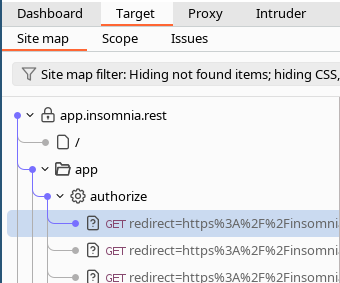
\includegraphics[width=1.0\linewidth]{images/burp_suite_site_map.png}
	\caption{Burp Suite Site Map}
	\label{fig:placeholder}
\end{figure}

\section{Identifying technologies, Services and Versions}

After mapping the domain, the next step was to identify the technologies and services in use, as well as their respective versions. This information is particularly valuable because outdated or vulnerable versions of software can often be directly linked to known vulnerabilities and CVEs.
To collect this data, we relied on multiple tools in order to cross-check and validate results. The main tools we used were httpx, nuclei, Nmap, and the Wappalyzer browser extension.
For example, httpx was used to extract basic information such as server headers, technologies, and response metadata:

\begin{lstlisting}[style=bash]
httpx -l targets.txt -tech-detect -status-code -title -o httpx_out.txt
\end{lstlisting}

We also used Nmap for service and version detection when applicable:

\begin{lstlisting}[style=bash]
nmap -sV -Pn target.com
\end{lstlisting}

Nuclei was used to identify known technologies and misconfigurations through template-based scanning:

\begin{lstlisting}[style=bash]
nuclei -l targets.txt -t technologies/ -o nuclei_out.txt
\end{lstlisting}

Additionally, Wappalyzer was used during manual exploration to confirm technologies detected by automated tools. Using multiple tools helped reduce false positives and gave us a more reliable understanding of the target environment.

\section{Subdomain Enumeration}

Once we moved to the IBM program, our previous reconnaissance approach was no longer sufficient. The scope included a wildcard domain (*.ibm.com), which required us to enumerate as many subdomains as possible.
To accomplish this, we used a variety of subdomain enumeration tools, including subfinder, chaos, assetfinder, waybackurls, and findomain. Initially, we relied only on subfinder, which produced approximately 15,000 subdomains. While this number was already large, we suspected that many more subdomains existed.
We then introduced additional tools and merged their outputs, carefully removing duplicates, invalid entries, subdomains not ending in ibm.com, and entries containing wildcard characters. By combining the results from subfinder, findomain, and assetfinder, the total number of discovered subdomains increased to approximately 41,000.
Encouraged by this significant increase, we continued adding more tools to the enumeration process. In the end, using all the tools mentioned above, we were able to identify approximately 352,000 unique subdomains.

\section{Finding the High-Signal Subdomains}

Enumerating hundreds of thousands of subdomains is useful, but it is not feasible to manually analyze all of them. Therefore, filtering and prioritization became a critical step.
We began by running httpx against the full list of enumerated subdomains:

\begin{lstlisting}[style=bash]
httpx -l subdomains.txt -o alive.txt
\end{lstlisting}

This step alone reduced the list to around 2,000 valid subdomains, as the majority of the enumerated entries did not resolve via DNS. At the same time, httpx provided additional metadata that we could later analyze to identify potential targets.
Initially, we made a mistake that we later recognized as overfiltering. For example, we removed subdomains that redirected to the same final URL, assuming they were equivalent. Later, we learned that this assumption was incorrect. Many subdomains redirected to identical login pages with the same status code, response size, and URL, yet differed in important aspects such as cookies and backend behavior.
A similar misconception occurred when dealing with IP addresses. We initially assumed that subdomains resolving to the same IP were effectively the same target, overlooking the fact that virtual hosts can serve different applications on the same IP address.
These mistakes taught us an important lesson about filtering. Aggressive filtering can easily remove valuable targets. To address this, we started clustering subdomains that shared the same IP address or final URL instead of discarding them outright. This allowed us to manually inspect these clusters and avoid missing potential attack surfaces.
We also experimented with Subwiz, an AI-based tool designed to identify high signal subdomains. However, in our case, it only returned two very generic subdomains that did not provide any meaningful value, so it was not particularly useful for our workflow.

\section{Automation}

Towards the end of the project, we realized that many of the early reconnaissance steps were repeated across different programs. This motivated us to start developing an automation script in Python to orchestrate the execution of multiple tools and manage their outputs in a structured way.
Due to time constraints, the script is still in an early stage of development. At its current state, it automates subdomain enumeration using the previously mentioned tools and performs basic filtering and clustering using httpx. However, even this limited functionality significantly reduced manual effort and improved consistency.
As we plan to continue working on Bug Bounties beyond this project, we also intend to incrementally improve this tool. Future improvements include more advanced filtering logic, better prioritization of results, and the integration of technology and service identification. The current version of the script will be submitted together with this report.

\chapter{Bug found on IBM program}

\section{Initial Discovery }

The assessment began with the identification of the subdomain:

\texttt{https://wmapigw-x7k-gw.d-v12b.apiconnect.dev.automation.ibm.com/} discovered in the reconnaissance phase. This subdomain appeared to host an IBM webMethods API Gateway and Integration Server deployment. At the time of discovery, no authentication had yet been performed, and the system was treated as an external-facing asset.

The initial interaction with the discovered subdomain focused on basic surface enumeration in order to identify exposed functionality. A directory and endpoint discovery phase was conducted using the \texttt{ffuf} fuzzing tool in combination with a commonly used wordlist (\texttt{common.txt}).

Through this fuzzing process, two unauthenticated endpoints were identified: \texttt{/health} and \texttt{/metrics}.

The \texttt{/health} endpoint returned standard liveness and readiness information, confirming that the service was running correctly. More notably, the \texttt{/metrics} endpoint returned structured operational data, including internal server identifiers, component-level metrics, and runtime information. Although the metrics endpoint did not expose credentials or secrets in the traditional sense, it returned detailed operational information such as CPU usage, memory consumption, uptime, thread statistics, and component-level identifiers. This type of data is typically consumed by internal monitoring systems  and is not intended to be accessible from untrusted networks.

The fact that the \texttt{/metrics} endpoint was reachable without authentication strongly suggested a configuration intended for internal observability that had been inadvertently exposed publicly. Even in the absence of explicit secrets, such operational metrics provide valuable reconnaissance information by confirming the underlying technology stack, deployment model, and runtime characteristics of the server. This exposure therefore indicated a likely misconfiguration at the perimeter or access-control level, warranting further investigation of the host.


We proceeded with light enumeration using multiple wordlists to identify additional exposed paths and interfaces. While most attempts returned access-denied responses, the presence of management-related endpoints suggested that authentication might be enforced at a higher layer rather than through network isolation.

At this stage, we considered the likelihood of default or well-known credentials being in use. This assumption was not arbitrary. webMethods installations are known to ship with predefined administrative accounts, most notably the \texttt{Administrator} user. In development, testing, academic, and misconfigured production environments, it is not uncommon for these default credentials to remain unchanged, especially when the system is deployed automatically through container images or platform templates.

Based on these factors, we attempted authentication using the default \texttt{Administrator} account with common documented default passwords associated with webMethods installations, in this case, the password  \texttt{manage}. This approach was validated when authentication succeeded, confirming that default administrative credentials were still active.

The successful login marked a critical transition point in the assessment: what initially appeared to be a passive information exposure escalated into full administrative access. Importantly, this outcome was not the result of brute force or credential guessing at scale, but rather of informed reasoning based on exposed system metadata, known product behavior, and configuration hygiene weaknesses.


\clearpage
\section{Initial Assessment of Server Environment and Dashboard Exploration}

After obtaining access to the webMethods administrative dashboard, our first objective was to understand the underlying system and the environment hosting the integration services. The dashboard provided detailed server information, which allowed us to characterize the deployment and assess potential security boundaries.

We systematically explored the available sections of the dashboard, reviewing execution logs, server statistics, and monitoring data. The logs showed little to no evidence of active API traffic or recent service execution beyond routine internal processes. Similarly, runtime statistics indicated minimal resource utilization, with low CPU and memory activity. These observations suggested that the platform was either idle, underutilized, or not actively serving production workloads.

Further inspection of server uptime information revealed that the instance had been running for approximately four days. This relatively short uptime, combined with the lack of meaningful operational activity, reinforced the hypothesis that the environment was not in active use. It appeared more consistent with a test, staging, or abandoned deployment rather than a production-critical system.

\subsection{System Properties and Environment}

The server exposed comprehensive runtime and environment properties, including:

\begin{itemize}
	\item \textbf{Architecture:} amd64
	\item \textbf{CPU:} Intel(R) Xeon(R) Platinum 8175M CPU @ 2.50GHz, 2 cores
	\item \textbf{Memory:} 7 GB
	\item \textbf{Operating System:} Linux 5.14.0-427.94.1.el9\_4.x86\_64
	\item \textbf{Hostname:} wmapigw-x7k-apigateway-0.wmapigw-x7k-apigateway-all.wmapigw-x7k.svc.cluster.local
	\item \textbf{OS Service Pack:} unknown
\end{itemize}

The system was running a containerized or orchestrated environment, likely managed via Kubernetes, as indicated by the hostname structure and the ephemeral nature of configuration changes.

\subsection{Software Stack}

The platform was operating on Microservices Runtime version 12.1.0.0, with Java 21.0.9 (Eclipse OpenJ9 VM) provided by IBM, and multiple core libraries loaded from standard Integration Server and Common directories. The Java runtime was located at \texttt{/opt/webmethods/jvm/jvm} and was configured without Semeru FIPS enabled. The server process ran under ID 38 with the instance named \texttt{Default}, and the working directory was \texttt{/opt/webmethods/IntegrationServer}.

\clearpage
\subsection{Dashboard Observations}

Within the dashboard, we observed:

\begin{itemize}
	\item CPU and memory utilization
	\item Disk usage and free space
	\item Java heap and thread metrics
	\item Package information and loaded libraries
\end{itemize}

\begin{figure}[h]
	\centering
	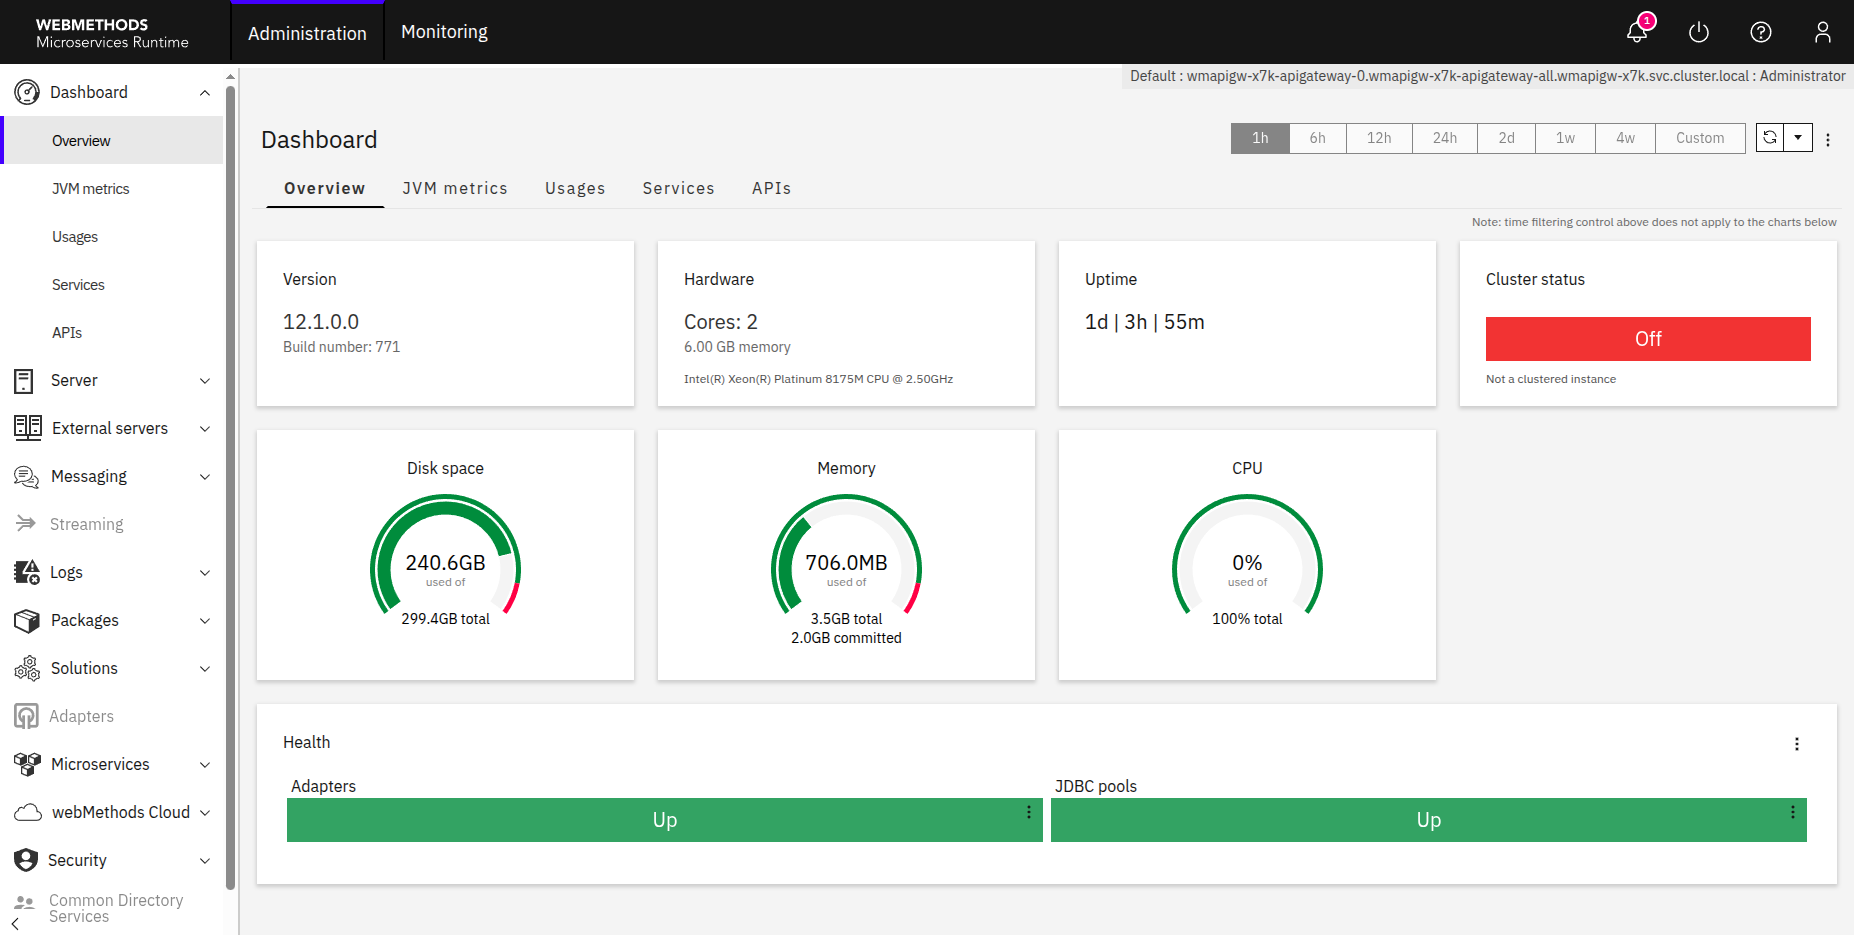
\includegraphics[width=1.0\linewidth]{images/Screenshot from 2026-02-04 15-34-01.png}
	\caption{Webmethods dashboard}
	\label{fig:placeholder}
\end{figure}


\subsection{Assessment Goals}

Given the exposure of internal metrics and server configuration details, our primary objective became privilege escalation beyond the application layer. Specifically, we aimed to determine whether administrative access to the webMethods dashboard could be abused to gain broader visibility or control over the underlying server or container infrastructure. This included exploring whether built-in management services could be leveraged to access the filesystem, interact with operating system resources, or pivot toward other components of the surrounding infrastructure.

\clearpage
\section{Exploitation Potential}

The webMethods administrative dashboard serves as the central interface to manage and monitor the integration server environment. It exposes a hierarchy of \textit{packages}, \textit{services}, and other runtime components that collectively orchestrate enterprise-level microservices and API workflows.

\subsection{Packages and Services}

Within the dashboard:

\begin{itemize}
	\item \textbf{Packages:} Collections of pre-configured services, libraries, and configurations. Packages often correspond to functional modules such as API Gateway, Cloud Integration, or Analytics components.
	\item \textbf{Services:} Individual operations provided by packages. Services can handle tasks such as processing requests, transforming data, interacting with databases, or managing message queues.
\end{itemize}

Each package and service runs directly on the host OS through the Java-based Integration Server, which interprets and executes these operations in the context of the running Java Virtual Machine. This architecture allows services to access system resources, including filesystem paths, network interfaces, and configuration files, depending on permissions.


\subsection{Security Context and Exploitation Potential}

The integration server instance was observed to run under a non-root user account, as is typical for production webMethods deployments. This was inferred from the service’s limited file access permissions and the lack of root-level filesystem paths in the displayed environment.

Because the packages and services operate on the OS level through the JVM, there is potential for exploitation if the server misconfigurations or default credentials allow access to administrative functions.
\clearpage
\section{Attempted Runtime Modification of File Access Controls}
The Integration Server exposes a configuration interface called \emph{Extended Settings}, which allows administrators to modify internal key--value parameters governing server behavior. Unlike services or packages, these settings act as a live registry that directly influences security enforcement without necessarily requiring a restart.

\subsection{Targeting File System Access Controls}

During earlier attempts, multiple file-related services such as \texttt{pub.file:getFile},

\texttt{pub.file:stringToFile}, \texttt{pub.file:copyFile}, etc, consistently failed with access control errors. These errors referenced the server’s file access control mechanism, specifically indicating that requested paths were not included in the \texttt{allowedWritePaths} or \texttt{allowedReadPaths} defined by the system configuration.

This behavior suggested that file system access was governed by a centralized policy rather than service-specific logic. As a result, the team investigated whether these restrictions could be modified dynamically through the Extended Settings interface.

\subsection{Runtime Security Policy Modification Attempt}

The following configuration key was identified as directly related to file system protection:

\begin{itemize}
	\item \texttt{watt.server.fileAccessControl.enabled}
\end{itemize}

An attempt was made to weaken or disable file access enforcement by modifying this parameter at runtime. The configuration was changed to disable file access control entirely and to permit unrestricted access to the filesystem root. Specifically, file access control was set to disabled.

After applying this change, the server accepted the new configuration without immediate error. This indicated that the platform allows administrators to alter critical security controls dynamically while the server is running.
\begin{figure}[h]
	\centering
	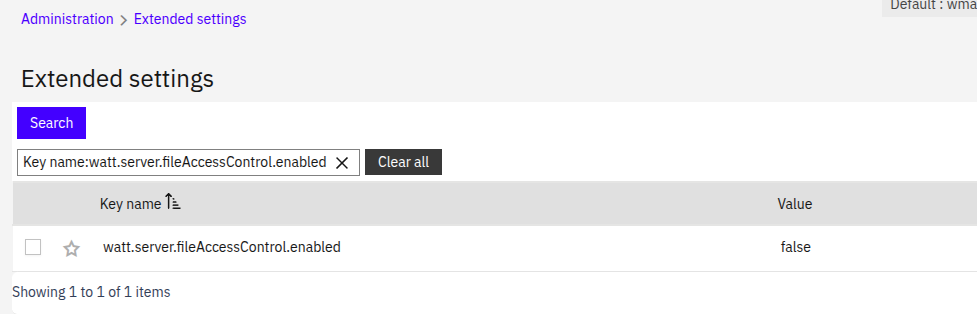
\includegraphics[width=0.9\linewidth]{images/Screenshot from 2026-02-05 19-07-29.png}
	\caption{FileAccessControl paremeter value on extended settings}
	\label{fig:placeholder}
\end{figure}
\subsection{Verification Attempts}

Following the configuration changes, the team attempted to validate whether the modified policy had taken effect by invoking \texttt{pub.file:stringToFile}. The test involved writing a simple text file to a directory that had previously been denied, such as \texttt{/tmp}. The service execution confirmed that the service itself was operational; however, the expected relaxation of file system restrictions did not persist reliably.

Additional attempts were made to read sensitive configuration files, such as user configuration data, using \texttt{pub.file:getFile}. These attempts continued to be blocked or inconsistently enforced, suggesting partial or transient application of the modified policy.

\subsection{Effect of Server Restart}

To determine whether the configuration changes required a restart to fully apply, we induced a server restart. Upon restart, all modified Extended Settings reverted to their default values. The previously altered file access control parameters were reset, and the restrictive file access policies were reinstated.

This behavior demonstrated that the environment is effectively stateless or immutable across restarts, with runtime configuration changes not being persisted. As a result, any temporary weakening of file system security would only be effective during the active lifecycle of the running instance.

\subsection{Outcome of the Attempt}

This attempt did not result in a successful bypass of the file system access restrictions. Although several security-related server properties were modified through the administrative interface, these changes did not lead to the intended ability to read or write restricted paths. Access denials continued to occur across multiple file-related services.

A definitive observation was made regarding configuration persistence. After restarting the server, all modified properties were reverted to their default values, indicating that configuration state is externally managed and not persisted locally.


\clearpage
\section{Attempts to Execute Operating System Commands and Inspect API Gateway Interfaces}

After establishing that direct file system access was heavily restricted and that runtime configuration changes were ephemeral, the next phase of exploration focused on two related goals: interacting with the API Gateway’s internal management interfaces and determining whether the Integration Server could be leveraged to execute operating system commands indirectly.

\subsection{Direct Access to API Gateway REST Interfaces}
An initial attempt was made to interact with the API Gateway management REST interface by invoking it through the Integration Server itself, using the built-in \texttt{pub.client:http} service. This service allows the server to issue outbound HTTP requests and is commonly used for backend integrations.

The target URL used in this attempt was:\\
\texttt{https://wmapigw-x7k-apigateway-0.wmapigw-x7k-apigateway-all.wmapigw-x7k.svc.cluster.local}

The objective of this step was to determine whether administrative access to the API Gateway could be achieved indirectly by issuing internal requests from within the cluster context, rather than accessing the endpoint directly from an external client. Successful access would have allowed enumeration and manipulation of deployed APIs and potentially enabled further privilege escalation within the platform.

Despite multiple attempts and variations using credentials available to the Integration Server session, all requests issued via \texttt{pub.client:http} resulted in HTTP 401 (Unauthorized) responses. This indicated that the API Gateway REST interface enforces authentication controls that are independent of the Integration Server dashboard session and could not be bypassed using internal service-to-service requests.

As a result, this path was abandoned, and further efforts focused on exploiting callable Integration Server services and file system interactions rather than the API Gateway REST layer.


\subsection{Exploration of Operating System Command Execution}
Following the unsuccessful attempt to access the API Gateway REST interface, attention shifted toward achieving operating system–level interaction through Integration Server services. Specifically, the built-in service \texttt{pub.utils:executeOSCommand} was tested. This service is intended to execute operating system commands from within the Integration Server context and, if misconfigured, can provide direct command execution on the host.

The goal of this attempt was to determine whether administrative access to the dashboard could be escalated into arbitrary command execution on the underlying container or host operating system. A successful invocation would have enabled direct inspection of the filesystem, process environment, and potentially outbound network access.

Multiple invocations of \texttt{pub.utils:executeOSCommand} were attempted using simple commands (e.g., \texttt{ls}, \texttt{env}, \texttt{cat}) and default parameter structures. However, all attempts failed with runtime errors indicating strict input validation, including repeated messages stating that the \texttt{environment} parameter was not of type \texttt{String[]}.

This behavior indicated that the service was active but constrained by strict parameter typing and additional execution restrictions, likely enforced through an allowlist defined in the \texttt{OSCommands.cnf} configuration. As a result, arbitrary command execution was not achievable through this service, and this attack path was abandoned in favor of file-based service exploration.


\subsection{Whitelisting and Command Restriction Mechanisms}

Further analysis revealed that operating system command execution within the Integration Server is governed by a configuration file that explicitly defines which commands are permitted. This design prevents arbitrary command execution even when the corresponding service is accessible.

To better understand the scope of this restriction, an attempt was made to locate and read the configuration file responsible for defining allowed commands. The file resides within the server’s package configuration directory and contains the list of commands deemed safe by the platform.

However, attempts to read this file using file access services were constrained by the same file access control mechanisms encountered earlier. As a result, the contents of the allow-list could not be reliably retrieved at this stage, limiting the ability to tailor command execution attempts to permitted binaries.

\subsection{Outcome of the Attempt}

These attempts did not result in successful execution of arbitrary operating system commands or direct interaction with the API Gateway’s management APIs. Instead, they demonstrated that:

\begin{itemize}
	\item Internal API Gateway REST endpoints were reachable but properly protected by authentication.
	\item Operating system command execution services were present but constrained by strict input validation and command allow-lists.
	\item Even administrative-level access within the dashboard did not equate to unrestricted control over the underlying operating system.
\end{itemize}

This phase of the investigation clarified that direct command execution was unlikely to be the primary attack vector and that further progress would require identifying inconsistencies or edge cases in how file access and service-level permissions were enforced.
\clearpage
\section{Access to Cryptographic Material and Limitations of Binary File Exfiltration}

As file access attempts expanded beyond configuration files and logs, attention shifted toward cryptographic material used by the API Gateway and Integration Server. During this phase, a Java KeyStore (JKS) file associated with the API Gateway was identified and successfully accessed through the available \texttt{pub.file:getFile} service.

\subsection{Discovery of the API Gateway Keystore}

Using the mentioned service, it was possible to read the contents of the following file:

\begin{verbatim}
/opt/webmethods/common/conf/DEFAULT_APIGW_KEYSTORE/keystore.jks
\end{verbatim}
At this point, the investigation shifted toward probing the filesystem for sensitive artifacts that could be accessed through available file-related services. The goal was to identify whether critical configuration files, credentials, or cryptographic material were exposed. Known high-value locations commonly used by webMethods and API Gateway deployments were therefore tested to assess the extent of unintended access to confidential data.

This file is a Java KeyStore and is used by the API Gateway to store private keys and certificates for TLS communication. From a security perspective, this file represents a highly sensitive asset, as it may contain private keys that identify the service within the cluster and establish trust relationships with other internal components.

When the file was retrieved through the dashboard, its contents were displayed directly in the browser as text. The output appeared as unreadable or garbled characters, which initially suggested an encoding issue or corruption during retrieval.

\subsection{Nature of the Retrieved Data}

The apparent corruption was not due to an error in retrieval, but rather to the nature of the file itself. A Java KeyStore is a binary format, and the dashboard attempted to render it as plain text. As a result, the raw binary bytes were interpreted as characters, producing unintelligible output.

Despite this limitation, visual inspection of the output revealed recognizable strings embedded within the binary data, including aliases and identifiers associated with the API Gateway and its internal certificate authority. These artifacts confirmed that the file was authentic and that sensitive cryptographic material was indeed being exposed at the file access layer.

This demonstrated that, from an access control standpoint, the server did not adequately prevent read access to critical cryptographic assets, even though practical exploitation was hindered by tooling constraints.

\begin{figure}[h]
	\centering
	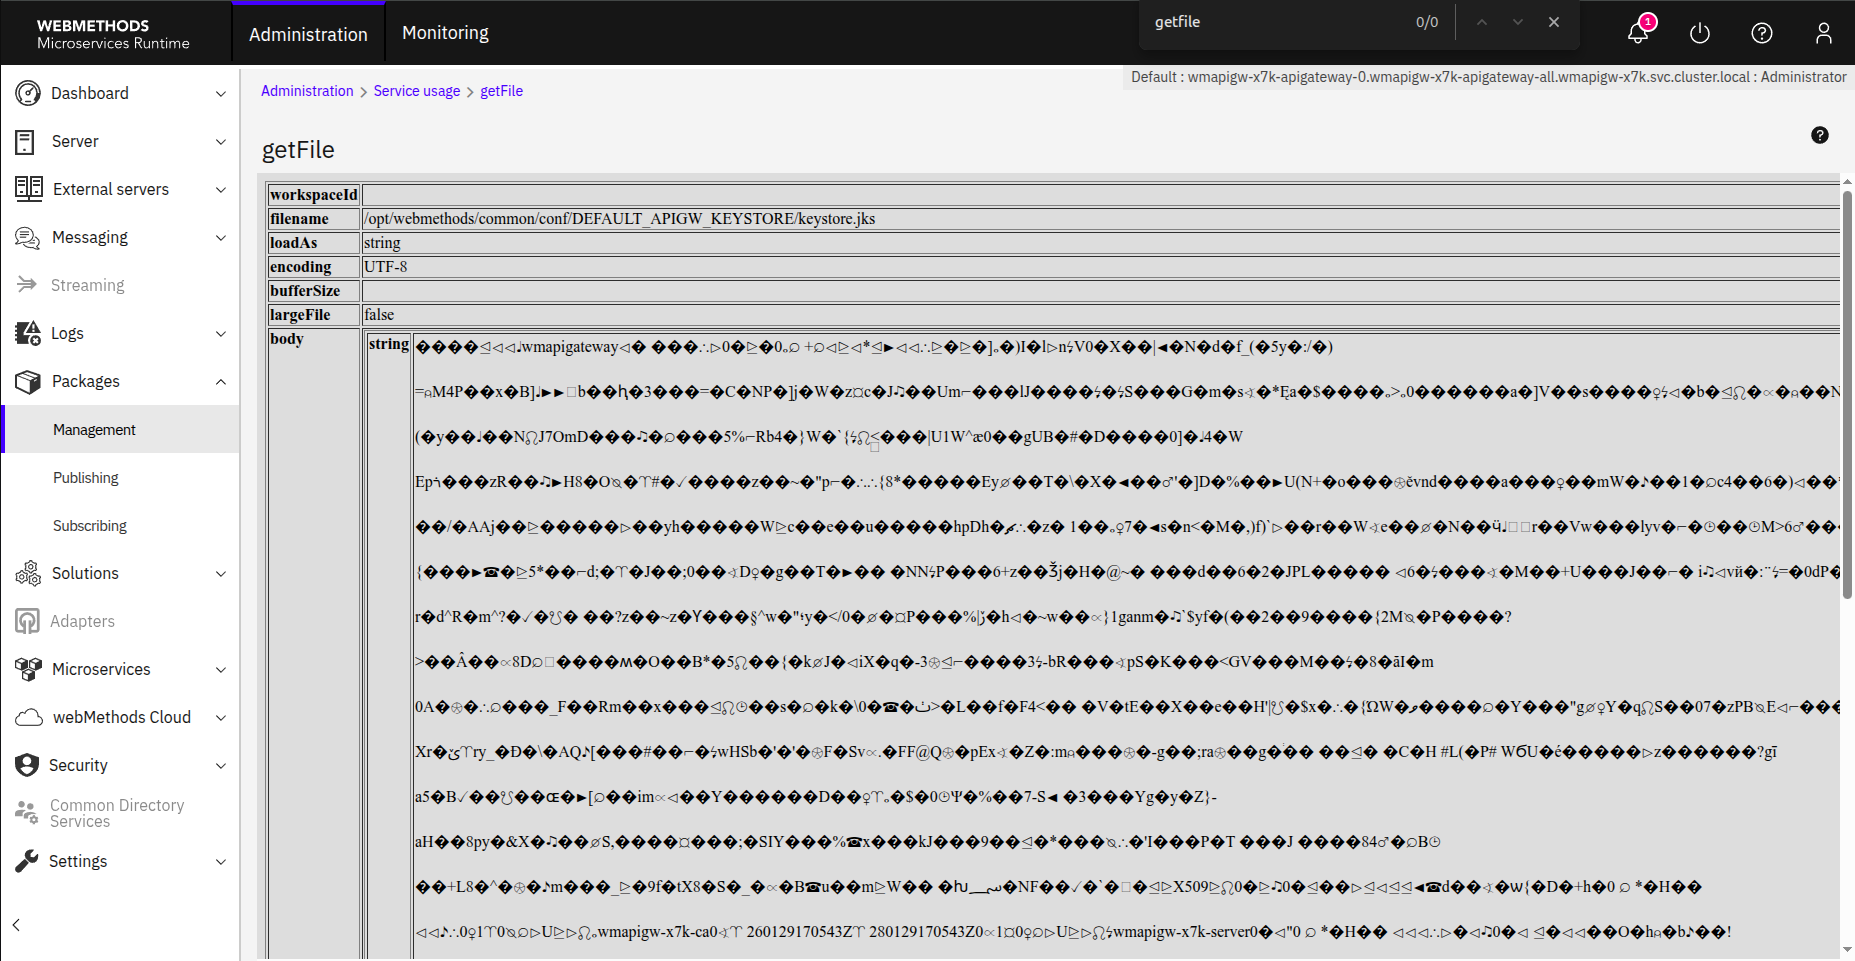
\includegraphics[width=0.9\linewidth]{images/Screenshot from 2026-02-05 19-03-11.png}
	\caption{Get file service output}
	\label{fig:placeholder}
\end{figure}

\subsection{Attempts to Preserve Binary Integrity}

Recognizing that copy-pasting or visually inspecting the file would irreversibly corrupt the data, multiple attempts were made to preserve the binary integrity of the keystore. These included:

\begin{itemize}
	\item Attempting to retrieve the file using alternative file services.
	\item Attempting to copy the file to a different location within the file system.
	\item Attempting to re-write the retrieved data back to disk in a controlled manner.
\end{itemize}

However, these attempts were largely unsuccessful. File copy and move operations were frequently blocked by the same path-based restrictions encountered earlier. Additionally, services capable of writing files required correctly structured binary input, which could not be reconstructed from the textual representation shown in the dashboard.

As a result, while the keystore could be read, it could not be reliably reconstructed into a valid binary file suitable for offline analysis or cryptographic tooling.

\subsection{Impact and Practical Limitations}

From a theoretical security perspective, exposure of a keystore file represents a critical weakness. Such a file may contain private keys capable of authenticating the service to other internal components, enabling impersonation or man-in-the-middle attacks within the cluster.

In practice, however, the inability to export the keystore in a usable binary form significantly limited immediate exploitation. The environment’s restrictions on file writing and binary handling prevented the keystore from being converted into a functional artifact outside the system.

\clearpage
\section{File Access Control Enforcement and Inconsistent Path Restrictions}

At this stage of the assessment, file-system interaction became a central focus. Previously identified file access services were reused to systematically test which paths could be read or blocked by the platform’s access controls, with particular attention given to locations likely to contain configuration data, credentials, or runtime secrets.


\subsection{Overview of File Access Controls}

The server enforces file-system restrictions through a path-based allowlist mechanism defined in its file access control configuration. When attempting to access files outside of explicitly permitted directories, the server consistently returned errors similar to the following:

\begin{verbatim}
[ISS.0086.9263] Specified path
[/opt/webmethods/IntegrationServer/config/fileAccessControl.xml]
is not on the [allowedWritePaths] allowed list in the
fileAccessControl configuration file
\end{verbatim}

These errors were encountered across multiple file-related services, including:
\begin{itemize}
	\item \texttt{pub.file:getFile}
	\item \texttt{pub.file:copyFile}
	\item \texttt{pub.file:moveFile}
	\item \texttt{pub.file:stringToFile}
\end{itemize}

As a result, many high-value directories, such as configuration and binary paths, were effectively blocked, significantly constraining further exploitation attempts.

\subsection{Impact on File Injection Attempts}

In addition to reading files, attempts were made to inject custom files into the system using \texttt{pub.file:stringToFile}. For example, writing a proof-of-concept script to a binary directory resulted in the following error:

\begin{verbatim}
[ISS.0086.9263] Specified path
[/opt/webmethods/IntegrationServer/bin/bounty_proof.sh]
is not on the [allowedWritePaths] allowed list in the
fileAccessControl configuration file
\end{verbatim}

These restrictions prevented arbitrary file creation in execution-relevant locations, effectively blocking common post-exploitation techniques such as script placement or binary replacement.

\subsection{Inconsistent Enforcement Across Services}

Despite the presence of file access controls, their enforcement was not uniform across all services. In several cases, the same path was treated differently depending on which service was used.

A notable example involved the path:

\begin{verbatim}
/proc/1/environ
\end{verbatim}

This file could not be accessed or copied using services such as \texttt{copyFile} or \texttt{moveFile}, as those operations were blocked by path restrictions. However, when accessed using \texttt{pub.file:getFile}, the request succeeded and returned the file contents.

This inconsistency indicates that the file access control layer is applied unevenly across different file-handling services. While some operations correctly enforced the configured restrictions, others allowed access to sensitive system files that should not have been readable under any circumstances.

\subsection{Security Implications}

The inconsistent behavior of the file access control mechanism introduces a subtle but critical weakness. Although many direct exploitation paths were blocked, the ability to selectively read files outside the intended allowlist undermines the effectiveness of the security model.

From an attacker’s perspective, this creates opportunities to probe the file system service-by-service, identifying which operations bypass restrictions and which do not. Even when write access is properly constrained, unauthorized read access, particularly to pseudo, files under \texttt{/proc}, can expose sensitive runtime information about the underlying container or host environment.

\clearpage
\section{Final Exploitation: Disclosure of Runtime Secrets via \texttt{/proc/1/environ}}

After extensive experimentation with the available file-related services, a critical inconsistency was identified in the enforcement of file access controls. While several sensitive directories under \texttt{/opt/webmethods/IntegrationServer/} were correctly protected by the \texttt{fileAccessControl} mechanism, the restrictions were not applied uniformly across all services. In particular, the service \texttt{pub.file:getFile} exhibited behavior that differed from other file manipulation services such as \texttt{pub.file:copyFile}, \texttt{pub.file:moveFile}, and \texttt{pub.file:stringToFile}.

During testing, most attempts to access protected filesystem paths resulted in explicit access-denied errors. However, when \texttt{pub.file:getFile} was invoked with the path \texttt{/proc/1/environ}, the service successfully returned the contents of the file. This path belongs to the Linux \texttt{/proc} pseudo-filesystem and exposes the environment variables of process ID 1. In a containerized deployment, process ID 1 corresponds to the main application process running inside the pod.

The ability to read \texttt{/proc/1/environ} represents a critical security failure, as this file contains all environment variables injected into the container at runtime. These variables are commonly used to store secrets and configuration values that are not intended to be accessible from the application layer. The returned output contained a large volume of sensitive information in plaintext.

A subset of the environment variables returned from \texttt{/proc/1/environ}, reformatted for readability, is shown below. These values demonstrate the presence of plaintext credentials, cryptographic secrets, and cloud configuration injected at runtime.

\begin{verbatim}
--- Administrative & Authentication Secrets ---
apigw_users_AdminUser_password=[REDACTED]
apigw_ports_1_regUsername=[REDACTED]
apigw_ports_1_regPassword=[REDACTED]
SAG_IS_MASTER_PASSWORD_KEY=[REDACTED]

--- Keystore / Truststore Secrets ---
keystore.DEFAULT_APIGW_KEYSTORE.ksPassword=manage
keystore.DEFAULT_APIGW_KEYSTORE.keyAlias.wmapigateway.keyAliasPassword=manage
keystore.EXT_APIGW_KEYSTORE.ksPassword=manage
keystore.EXT_APIGW_KEYSTORE.keyAlias.ext-wmapigateway.keyAliasPassword=manage
truststore.DEFAULT_APIGW_TRUSTSTORE.ksPassword=manage
apigw_cluster_ignite_keystorePassword=manage
apigw_cluster_ignite_truststorePassword=manage
apigw_dataStore_https_keystorePassword=manage
apigw_dataStore_https_truststorePassword=manage
apigw_ui_https_keystorePass=manage
apigw_ui_https_keyPass=manage

--- Cloud Credentials (AWS) ---
apigw_aws_os_access_key=[REDACTED]
apigw_aws_os_secret_key=[REDACTED]
apigw_aws_region=us-east-1
apigw_aws_os_enabled=true
apigw_aws_os_service_name=es
apigw_aws_os_role_arn=arn:aws:iam::091790783357:role/AP_B_G_SSRE_apic_serviceRole_apic-d-v12b-analytics-os-role

--- Internal Cluster & Management Endpoints ---
apigw_mgmt_endpoint=https://wmapigw-x7k-mgmt.d-v12b.apiconnect.dev.automation.ibm.com
API_GW_HOME_PAGE=https://wmapigw-x7k-ui.d-v12b.apiconnect.dev.automation.ibm.com/apigatewayui/
apigw_dataStore_hosts=vpc-apic-d-v12b-apigw-ez7myxfhrkdmxh6ggj4xgqxxwy.us-east-1.es.amazonaws.com

--- Kubernetes / Container Metadata ---
POD_NAME=wmapigw-x7k-apigateway-0
POD_NAMESPACE=wmapigw-x7k
POD_UID=6f251885-d92b-4cce-a6ed-edaf750b3750
POD_IP=172.21.18.179
KUBERNETES_SERVICE_HOST=172.30.0.1
KUBERNETES_SERVICE_PORT=443

--- Runtime & Platform Information ---
JAVA_MIN_MEM=2048M
JAVA_MAX_MEM=3584M
JAVA_HOME=/opt/webmethods/jvm/jvm
SAG_HOME=/opt/webmethods
APIC_CLOUD_TYPE=AWS_MT
container=oci
FIPS_ENABLED=false
\end{verbatim}


Notably, this exploitation step did not require operating system command execution, package installation, or container escape. The attack relied solely on reading a single file via a built-in service that was already accessible to the authenticated user. The root cause was an incomplete and inconsistent application of file access restrictions, which failed to account for sensitive pseudo-filesystem paths such as \texttt{/proc}.

The successful retrieval of \texttt{/proc/1/environ} marked the decisive point of compromise. At this stage, full control over the API Gateway environment was effectively achieved, alongside exposure of cryptographic material and cloud credentials capable of impacting the wider infrastructure.

\subsection{Critical Impact of Disclosed Secrets}

The disclosure of these runtime secrets represents a critical and high-impact security failure. The exposed environment variables included valid AWS access keys and secret keys associated with the API Gateway’s cloud role, enabling direct authentication against AWS-managed services such as OpenSearch without any further exploitation. Possession of these credentials allows an attacker to enumerate, read, modify, or delete cloud resources, access stored logs and analytics data, and potentially pivot to other services permitted by the attached IAM role. In parallel, the exposure of keystore and truststore passwords enables decryption and impersonation of internal TLS communications, undermining the trust model of the entire cluster. Combined with administrative user credentials and master encryption keys, these secrets effectively collapse the security boundary between application, container, and cloud infrastructure. As a result, a single misconfigured file read operation escalates from an application-layer issue into full compromise of cryptographic identity, management access, and underlying cloud infrastructure, placing the confidentiality, integrity, and availability of the entire environment at risk.

\subsection{Exposure of Cloud Inventory and Infrastructure Visibility}

The exposed cloud credentials provided broad visibility into the underlying AWS environment and revealed a large, mature, and actively used infrastructure. The accessible inventory included dozens of object storage buckets serving critical functions such as API Gateway backups, disaster recovery replicas, analytics offloading, image registries, logging pipelines, and internal data processing workflows. Multiple environments were identifiable, including development, testing, and production deployments, alongside supporting services for OpenSearch, Kafka connectors, FTP-based data exchange, and machine learning workloads. Metadata associated with compute resources indicated the presence of numerous running servers fulfilling roles such as API Gateway nodes, infrastructure components, worker nodes, and database-backed services.

While not all resources were enumerated here, the following table summarizes key types of assets and their intended purpose:

\begin{table}[h!]
	\centering
	\begin{tabular}{|l|p{10cm}|}
		\hline
		\textbf{Resource Type}           & \textbf{Purpose / Notes}                                                                                                                                                                                   \\ \hline

		S3 Buckets                       & Backups, disaster recovery replicas, analytics offloading, image registries, FTP pipelines, serverless deployments, step functions, and operational logs                                                   \\ \hline

		EC2 Instances                    & Running servers including API Gateway nodes, worker nodes, infrastructure servers, database-backed services for production, staging, and development environments, including 1 dedicated production server \\ \hline

		Machine Learning                 & SageMaker studios, ML pipelines, analytics offload and filtered analytics processing                                                                                                                       \\ \hline

		Logging / Monitoring             & CloudWatch export buckets, monitoring pipelines, logging of operational metrics and audit trails                                                                                                           \\ \hline

		Disaster Recovery / Backups      & Replica backups of production and staging environments, API Gateway backups, object storage for DR                                                                                                         \\ \hline

		Specialized Services             & Kafka connector S3 sinks, NLB debug buckets, FTP pipelines, serverless deployment buckets, codestar project buckets                                                                                        \\ \hline

		Application / Platform Artifacts & Step functions, image registries, build-cost tracking, analytics demos, and operational dependencies                                                                                                       \\ \hline
	\end{tabular}
\end{table}

\noindent
Access at this level would enable cloud-level lateral movement, data exfiltration from backup and analytics stores, tampering with operational artifacts, or interaction with live production systems. Although further actions, such as direct access to compute instances or modification of cloud resources, were technically feasible, no additional exploitation was performed at this stage, as proceeding further would likely exceed the intended assessment scope. This underscores the critical severity of the issue: a single application-layer flaw directly enabled exposure of credentials capable of impacting the broader cloud infrastructure.
\clearpage
\section{CVSS Severity Assessment}

The identified vulnerability was assigned a \textbf{Critical} severity rating with a base score of \textbf{9.8}.

\begin{quote}
	\textbf{CVSS v3.1 Vector:} \texttt{CVSS:3.1/AV:N/AC:L/PR:N/UI:N/S:U/C:H/I:H/A:H}
\end{quote}

This score reflects a remotely exploitable authentication misconfiguration that allowed unauthenticated attackers to obtain full administrative access to an internet-facing IBM webMethods Microservices Runtime instance. Exploitation required no prior privileges or user interaction and involved a low level of complexity due to the use of default credentials.

Successful exploitation resulted in complete compromise of the application environment, including unrestricted access to system configuration, runtime metadata, administrative functionality, and sensitive secrets. Notably, the compromised environment exposed valid cloud credentials associated with IBM-managed cloud infrastructure, enabling authenticated access to backend resources hosted on Amazon Web Services (AWS) and related cloud assets. This effectively extended the impact of the vulnerability from the application layer to the underlying cloud infrastructure.

The impact on confidentiality, integrity, and availability is considered high. Confidentiality was affected through access to sensitive application data and cloud credentials; integrity was compromised by the ability to modify application and cloud resource configurations; and availability was at risk due to the potential for service disruption or infrastructure-level impact. Taken together, these factors justify a Critical severity rating under CVSS v3.1.
\clearpage
\section{Remediation and Mitigation Recommendations}

To prevent recurrence of the identified vulnerability and reduce the risk of similar security issues across other environments, the following remediation and mitigation measures are recommended.

\subsection{Immediate Remediation Actions}

\begin{itemize}
	\item \textbf{Remove Default Credentials:} Ensure that all default usernames and passwords are disabled prior to deployment. Administrative accounts should require unique, strong credentials and enforce password complexity and rotation policies.

	\item \textbf{Restrict Administrative Interfaces:} Administrative dashboards and management endpoints should not be exposed to the public internet. Access should be limited through network controls such as private networking, IP allowlists, VPNs, or zero-trust access mechanisms.

	\item \textbf{Rotate Exposed Credentials:} Immediately revoke and rotate any cloud credentials that were accessible from the affected environment. This includes AWS credentials and any associated IBM cloud service credentials.
\end{itemize}

\subsection{Configuration and Deployment Hardening}

\begin{itemize}
	\item \textbf{Harden Application Configuration:} Disable unnecessary services, endpoints, and diagnostic interfaces (such as health or metrics endpoints) unless explicitly required. Where enabled, ensure that access is authenticated and authorized.

	\item \textbf{Secure Secret Management:} Application environments must not store long-lived cloud credentials in plaintext or accessible configuration contexts. Use a secure secret management solution with strict access controls and short-lived credentials where possible.

	\item \textbf{Least Privilege for Cloud Access:} Cloud identities used by application components should be scoped to the minimum permissions required. Avoid broad or administrative-level permissions for service accounts.
\end{itemize}

\subsection{Monitoring and Preventive Controls}

\begin{itemize}
	\item \textbf{Continuous Asset Discovery:} Implement regular scanning and inventory processes to identify exposed services, unused environments, and orphaned deployments that may be unintentionally accessible.

	\item \textbf{Security Monitoring and Alerting:} Enable logging and monitoring for authentication events, administrative access, and cloud API usage. Alerts should be configured for anomalous access patterns or credential misuse.

	\item \textbf{Security Reviews and Testing:} Incorporate routine security reviews and automated testing into deployment pipelines to detect misconfigurations such as default credentials, exposed management interfaces, and insecure secret handling prior to release.
\end{itemize}

Collectively, these measures address both the immediate cause of the vulnerability and the underlying systemic issues that allowed it to occur. Applying these recommendations will significantly reduce the likelihood and impact of similar vulnerabilities in the future.

\clearpage
\chapter{Conclusion}

This report documents a Critical security vulnerability affecting an internet-facing IBM webMethods Microservices Runtime environment. The issue originated from an authentication misconfiguration that allowed unauthenticated access using default administrative credentials. Once authenticated, full administrative control over the application environment was obtained without restriction.

The compromised environment exposed extensive system and runtime information and provided unrestricted access to administrative functionality. During further investigation, valid cloud credentials were discovered within the application context, enabling authenticated access to IBM-managed cloud infrastructure hosted on Amazon Web Services (AWS). This significantly expanded the impact of the vulnerability from an application-level compromise to a broader infrastructure-level security risk.

Although the affected instance appeared to be inactive at the time of discovery, the presence of default credentials and exposed cloud secrets represents a severe security failure with the potential for substantial harm. An attacker exploiting this vulnerability could gain persistent access to backend systems, access or manipulate sensitive data, and disrupt services at scale.

All testing activities were conducted in good faith and in accordance with IBM’s Safe Harbor Policy. No customer data was intentionally accessed, modified, or exfiltrated, and no actions were taken beyond what was necessary to validate the security impact of the vulnerability. This report is intended to support IBM’s coordinated vulnerability disclosure process and assist in the timely remediation of the identified issues.

Addressing this vulnerability requires not only the removal of default credentials and restriction of administrative access, but also a review of credential management practices, cloud access controls, and deployment exposure to ensure similar issues do not recur in other environments.

%%------------------------------- the end. ------------------------------------

\end{document}


